\documentclass[a4paper]{article}

\usepackage[english]{babel}
\usepackage[utf8x]{inputenc}
\usepackage{amsmath}
\usepackage{graphicx}
\usepackage[colorinlistoftodos]{todonotes}


%probs aliases	-------------------------------------------- [sec:probs]
\newcommand{\given}{\ensuremath{\,\mid\,}}
%\newcommand{\proba}[1]{\ensuremath{\mathcal{P}\left(\, #1 \,\right)}}
\newcommand{\proba}[2][]{\ensuremath{\mathcal{P}_{#1}\left(\, #2 \,\right)}}
\newcommand{\set}[1]{\ensuremath{\left\{\,#1\,\right\}}}
\newcommand{\age}{\ensuremath{\mathrm{age}}}
\newcommand{\fbump}{\ensuremath{f_\mathrm{b}}}
\newcommand{\data}{\ensuremath{\overrightarrow{d}}}
\newcommand{\dataerr}{\ensuremath{\overrightarrow{\sigma_d}}}
\newcommand{\nclobs}{\ensuremath{n_{c,obs}}}
\newcommand{\nclpred}{\ensuremath{n_{c,pred}}}
\newcommand{\birthrate}{\ensuremath{{\dot n}_{birth}}}
\newcommand{\tage}{\ensuremath{t_{age}}}
\newcommand{\Mi}{\ensuremath{M_{i}}}
\newcommand{\ts}{\ensuremath{\tilde{t}}} %survival time
\newcommand{\PI}{\ensuremath{\overrightarrow{\pi}}} %all dissol params
\newcommand{\T}{\ensuremath{\overrightarrow{\theta}}} %all cluster params 
\newcommand{\dif}{\ensuremath{\text{d}}} %differencial notation 


\title{Dissolution Notes}
\author{Morgan Fouesneau, Hans-Walter Rix \& David W. Hogg}

\begin{document}
\maketitle


The dissolution of star clusters in external galaxies can in principle be derived empirically from the analysis of the age distribution of detected clusters. If the clusters are destroyed rapidly in their host galaxy, the number of clusters will decrease rapidly with age, in the sense that there will be many fewer old than young clusters.
\begin{enumerate}
\item assume (or determine) a cluster formation history, it shapes of the distribution of the observed clusters.
\item Clusters fade with age due to stellar evolution for magnitude limited samples.
\item Incompleteness, which relates the true distribution of clusters to the observed one.
\item The accuracy of the age and mass determinations, which are based on the fitting of the photometric spectral energy distributions with cluster models.
\end{enumerate}

\medskip

We estimate the number of observed clusters $N(t, M)$ as a function of time $t$ and current mass $M$.


Under some assumptions, we have access to the 4th item, with $\T$ the intrinsic parameters of {\bf one} given cluster:
\begin{eqnarray}
\proba{\T_i = \set{age, mass...} \given \data_i,\, \dataerr_i} &=& \proba{ \data_i \given \T_i, \dataerr_i}\,\proba{\T_i}
\end{eqnarray}

So that for the ensemble of data $\data$:
\begin{eqnarray}
\proba{\T \given \data, \dataerr} &=& \prod_i \proba{\T_i \given \data_i}\\
                                                 &=& \prod_i \proba{ \data_i \given \T_i, \dataerr_i}\,\proba{\T_i}
\end{eqnarray}

Note that $\T$ represents the space of true clusters. The model has a sizeable set of meta-parameters, $\PI$, which describe the cluster formation history, the initial cluster mass function and the cluster dissolution process.


We can also presume that the completeness/selection function is also known in the age-mass space as $S(t, M)$.
\,\\

\medskip


{\bf Our goal is to sample the pdf of the parameters $\PI$, which describe the birth rate and the decay of a cluster {\it population} in light of our data \data on the observed cluster distribution 
$\nclobs(\tage,M)$ [with units of 1/time and 1/mass], that predicts the expected number of clusters in the sample in an interval $\Delta t,\Delta M$ around $(\tage,M)$ as $\langle N\rangle = \nclobs(\tage , M)\cdot \Delta t\Delta M$.}
\,\\
\begin{eqnarray}
\proba{\PI \given \data} &\propto& \proba{\data \given \PI}\proba{\PI}\\
                         &\propto& \proba{\PI}\,\int{\proba{\data \given \T}\,S(\T)\,\proba{\T\given \PI }d\T}
\end{eqnarray}

We can assume that we are working in the "true data" space "$\T$", in which there is no uncertainty on $t$ and $M$ of a given clusters. Using equation 5 above will bring us back into the real world.

Hence we need to explicit \proba{\T\given \PI }. We will only consider time and mass in the following, so that we define \proba{t, M \given \PI} as the marginalized probability:
\begin{eqnarray}
\proba{t, M \given \PI} &=& \idotsint \proba{\T \given \PI} \dif\theta_1 \cdots \dif\theta_n
\end{eqnarray}

The predicted number of observable clusters, $\nclobs(\tage, M)$, depends on the number of clusters formed at a given time which corresponds to the age of the cluster $t_{age}$ and its {\bf initial} mass $\Mi$ and how this particular cluster will lose mass with time $t$.
The number of observed clusters is the convolution of the true number of existing clusters with the selection function $S(\tage, M)$,
\begin{eqnarray}
\nclobs(\tage, M) &=& S(\tage, M)\,\nclpred(\tage, M) 
\end{eqnarray}
We now spell out explicitly the form of \nclpred, which actually depends on \PI as:

\begin{eqnarray}
\nclpred(\tage, M; \PI) &=& \int \birthrate(\tage, \Mi; \PI) \, \proba{\Mi \given \tage, M, \PI}\, \dif\Mi
\end{eqnarray}

We presume that \birthrate [units 1/time 1/mass] can be written as a separable function of the total cluster birth rate $CFR(t)$ a time $t$ {\bf ago}, and the normalized (birth) mass function, $\proba{\Mi}$:
\begin{eqnarray}
\birthrate(\tage, \Mi; \PI) &=& CFR(\tage; \PI) \, \proba{\Mi\given\PI}.
\end{eqnarray}

The observations give the present-day cluster mass, but the cluster-formation history is phrased in terms of the birth-mass $\Mi$. Since (at least in the Utrecht-world) cluster dissolution is an (in part)  stochastic process, there is no unique mapping between $M(\tage)$ and $\Mi$. This relation is therefore phrased in terms of the probability $\proba{\Mi \given t, M}$, which is non-trival. As cluster dissolution happens forward in time $\Mi \rightarrow M$, we make use of the Baye's theorem to express current current cluster mass as a function of its initial mass and its age:
\begin{eqnarray}
\proba{\Mi \given \tage, M, \PI} = \proba{M \given \tage, \Mi, \PI}\, \frac{\proba{\Mi\given\PI}}{\proba{M \given \tage, \PI}} \\
\proba{M\given \tage, \PI} = \int \proba{M\given \tage, \Mi, \PI }\, \proba{\Mi\given\PI }\, \dif\Mi
\end{eqnarray}

We need to express the stochastic process from the point $t_e$ (a few Myrs) when cluster starts its life with mass $\Mi$ to its present age \tage when it has a mass $M$.
A cluster evolves under internal processes until at some (stochastic) time $\ts$ an external potential, such as tidal interaction, spiral arms, etc, affects its quiet environment. The cluster will then be dominated by the disruption process and a faster mass loss.

This cluster dissolution process is characterized by four parameters, 
\begin{equation}
\PI_d \equiv (t_e,\gamma_e,\gamma_d,\tau),
\end{equation}
where $t_e\sim 1$~Myr is the age at which cluster evaporation begins, which then entails 
\begin{equation}
M(t; \PI)=M_i (t/t_e)^{-\gamma_e};
\end{equation}
after the (externally driven) dissolution sets in at time $\ts$, the mass evolves as 
\begin{equation}
M(t;\ts, \PI)=M(\ts )(t/\ts)^{-\gamma_d}.
\end{equation}

In a concern of simplifying the notations, we consider below $\PI_d$ to be part of $\PI$.
The current mass of a cluster $M$ is related to its initial mass $\Mi$ through a combination of internal mass loss and mass loss due to external factors, so called disruption.
As a result, we define the predicted current mass $M_{pred}$ of a cluster with a broken power-law as follow:
\begin{eqnarray}
M_{pred}(\tage, \Mi, \ts, \PI) = 
   \begin{cases}
   \Mi & \tage < t_e, \\
   \Mi \, \left(\frac{\tage}{t_e}\right)^{-\gamma_e}, & t_e < \tage < \ts, \\
   \Mi \, \left(\frac{\ts}{t_e}\right)^{-\gamma_e}\,\left(\frac{\tage}{\ts}\right)^{-\gamma_d}, & \ts < \tage,
   \end{cases}
\end{eqnarray}

where $t_e$ is the time at which internal processes are affecting the mass, $\ts$ the time at which the regime changes to include disruption processes, and $\gamma_e$, $\gamma_d$ the index of the decays, respectively. It comes that given a set $\set{\gamma_e, \gamma_d, t_e, \ts, \tage}$ of parameters, $M_{pred}$ is deterministically given as a function of the initial mass $M_i$. 
This statement leads us to write that
\begin{eqnarray}
\proba{M\given \Mi, \tage, \PI} =& \int_{t_e}^{\infty} \delta\left(M-M_{pred}( \tage, \Mi, \ts, \PI)\right)\proba{\ts\given\PI}\dif\ts
\end{eqnarray}

where $\proba{\ts \given \PI}$ characterizes the rate at which the rapid dissolution sets. The "survival" probability that no external perturbation has occured yet, and that hence rapid dissolution has not yet set in $p_s=\exp{(-t/\tau)}$, and the rate of dissolution onset \proba{\ts\given\tau} is its derivative:
\begin{eqnarray}
\proba{\ts\given\PI} & = &
1/\tau\,\, e^{-(\ts-t_e)/\tau}
\end{eqnarray}

In light of the three cases in Equation 12,  Equation 13 becomes

%\begin{eqnarray}
%\proba{M\given \Mi, \tage, \PI} =&\proba{\ts(M,\Mi,\tage,\PI) %\given \tau},
%\end{eqnarray}
%
\begin{eqnarray}
\proba{M\given \Mi, \tage, \PI} = \delta(M-M_{pred}(..))
   \begin{cases}
   0 & M/\Mi >1 \\
   e^{-(\tage-t_e)/\tau}& 1\ge M_{pred}/\Mi > \left(\frac{\tage}{t_e}\right)^{-\gamma_e}\\
   e^{-\ts(M-M_{pred})/\tau}& \left(\frac{\tage}{t_e}\right)^{-\gamma_e}>M_{pred}/\Mi\\
   %\exp{\left(-\tage/\tau\right)}& 1\ge M_{pred}/\Mi > \left(\frac{\tage}{t_e}\right)^{-\gamma_e}\\
   %\exp{\left(-\ts(M-M_{pred})/\tau\right)}& \left(\frac{\tage}{t_e}\right)^{-\gamma_e}>M_{pred}/\Mi\\
 0 & \left(\frac{\tage}{t_e}\right)^{-\gamma_d}>M/\Mi\\
%   \proba{\ts(M,\Mi,\tage,\PI) \given \tau} & TBD ,
   \end{cases}
\end{eqnarray}
%\todo{Take another look at the units of this expression -- I'm not completely following the limits}

 Here, the second line arose from 
\begin{eqnarray}
\int_{\tage}^{\infty}\proba{\ts\given\PI}\dif\ts = 
%\frac{1}{\tau} unit confusion HWR; double check
e^{-(\tage-t_e)/\tau}.
\end{eqnarray}
%where we have assumed that $t_e \ll \tage$.
For the last line, we need $\ts(M;\Mi,\tage,\PI)$ to be derived from Eq. 15 as
\begin{eqnarray}
\ts \left(M=M_{pred}; \tage, \Mi, \PI \right) = 
\left( \frac{M}{\Mi} \right)^{\gamma_e - \gamma_d} \, \frac{\tage^{\gamma_e}}{t_{e}^{\gamma_d}} & \left (\ts < \tage\right ).
\end{eqnarray}
This simplification arises because of the $\delta$-function in the integrand in Eq. 16 is only non-zero at a single $\ts$, which corresponds to $M=M_{pred}$.

\begin{figure}
  \begin{center}
    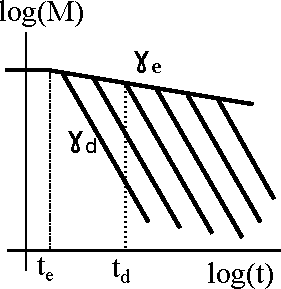
\includegraphics[width=0.5\textwidth]{schema.pdf}
  \end{center}
  \caption{Representation of the mass decay with time $M(t)$. We defined the decay as a broken power-law. The mass decays slowly under only internal processes from $t_e$ and strongly decreases as soon as the disruption is triggered at $\ts$.
	%\todo[inline]{revise according to notations and with only one scenario.}
  }
  \label{fig:mass_evol}
\end{figure}





Hence, we combine Eqs. 8, 9 \& 11 and the predicted number of clusters becomes:
\begin{eqnarray}
\nclpred(\tage, M, \PI) = CFR(\tage; \PI)\,\int \frac{\proba{\Mi\given\PI}^2}{\proba{M\given \tage,\PI}} \,\proba{M \given \tage, \Mi, \PI}\, d\Mi
\end{eqnarray}



\medskip

As a summary, we defined an ensemble of parameters, $\PI$, on which we will have priors:
\begin{eqnarray}
\PI =& & \set{ \PI_d:\, \gamma_e, \gamma_d, t_e, \tau}\,\nonumber \\
     &+& \,\set{\text{CIMF}:\,\alpha,\Mi^{min}, \Mi^{max}}\nonumber\\
     &+& \,\set{\text{CFR}:\,CFR(t)}
\end{eqnarray}

Looking back at the original equation (Eq.\,5):
\begin{eqnarray}
\proba{\PI \given \data} & \propto & \proba{\PI}\,\int{\proba{\data \given \T}\,S(\T)\,\proba{\T\given \PI }d\T}
\end{eqnarray}
\begin{itemize}
\item $\proba{\PI}$: prior on the population formation and dissolution parameters,
\item $\proba{\data \given \T}$: the likelihood of the ensemble of observed data with our cluster models, where $\T$ includes $(\tage,\,M)$, i.e., $\proba{\data \given \T} = \prod_i \proba{\data_i\given\T}$,
%\todo[inline]{we need to be clear, are $\vec{d}$ and $\vec\theta$ always about ensembles of clusters, or one cluster?}
\item $S(\T)$: our model of selection function (i.e., completeness and detection)
\item $\proba{\T\given \PI }\propto\proba{\tage, M\given \PI }$: the probability of the existence of a cluster of age $\tage$ and mass $M$ (given our assumptions),
\item $\proba{\tage, M\given \PI } = \nclpred(\tage, M; \PI) / \iint \nclpred(\tage, M; \PI)\dif\tage\dif M $, the number density of clusters of a given age and mass,
\item $\nclpred(\tage, M; \PI)$ as given by the integral given in Eq.\,21, which involves $\proba{\Mi\given\tage,M,\PI}$ (Eq.\,10) normalized through its integral on initial mass (Eq.\,11),
\item and, $\proba{M \given \tage,\Mi,\PI}$ as defined by Eq.\,15. 
\end{itemize}
\end{document}